\section{Environmental Disruptions, Evacuation, and Mobility Adaptation}
\label{sec:results_environment_disruptions}

Environmental disruptions are a useful test of whether an urban population model can distinguish a change in point-of-interest (POI) state from the behavioral response to that change. A POI may become unavailable, but this state alone does not determine what the population should do. A routine visit may be cancelled or redirected, a work or school trip may remain unmet because its destination is not substitutable, and a resident exposed at home may seek protection in a capacity-constrained shelter. These responses require different policies even when they originate from the same environmental observation.

The experiments in this section extend the routine-mobility baselines from Section~\ref{sec:results_routine_mobility} along two complementary paths. The first path applies a time-varying water-level series to home, activity, work, and school POIs, then evaluates trip suppression, destination substitution, and flood-aware commuting. The second path maps a static 5.30~m exposure estimate to the full-city population and evaluates evacuation toward shelters under capacity, response-rate, occupancy, distance, reallocation, and facility-failure variations. Together, the studies examine both disruption of ordinary movement and movement initiated specifically in response to exposure.

Following the distinction established in Chapter~\ref{chapter:proposed_model}, the water-level condition is represented as environment state, whereas suppression, substitution, evacuation, admission, and reallocation are plugin policies. More specifically, flood thresholds are stored in the POI attribute mappings $\bm{\alpha}_i$, the active flood condition is represented as a named cause in $C_i(t)$, and the response to an unavailable POI is determined by the handler that consumes the affected action. This separation allows the same environmental state change to produce different responses without assigning a universal flood behavior to the core environment.

\subsection{Environmental-Disruption Plugins}
\label{sec:environment_disruption_plugins}

Table~\ref{tbl:environment_disruption_plugin_contract} maps the extensions used in this section to the plugin contract from Section~\ref{sec:plugins}. The entries report the composed experimental behavior; components already introduced with routine mobility are repeated only to identify the parameters and lifecycle facilities activated by the disruption scenarios.

\begin{table}[ht]
\centering
\footnotesize
\setlength{\tabcolsep}{4pt}
\caption{Mapping of the environmental-disruption extensions to the plugin contract.}
\label{tbl:environment_disruption_plugin_contract}
\begin{tabularx}{\linewidth}{@{}p{2.7cm}p{3.7cm}X@{}}
\toprule
\textbf{Extension} & \textbf{Nonempty components} & \textbf{Role in the experiments} \\
\midrule
Water-level data
& $\bm{\theta}_{\mathrm{water}}$, $\Delta\Sigma_{\mathrm{water}}$, $\mathcal{H}_{\mathrm{water}}$
& Configures the water-level series and target POI types, declares the flood-threshold attribute convention, exposes water-level data, and adds or removes the \texttt{flood} cause in $C_i(t)$. \\
Popular Times
& $\bm{\theta}_{\mathrm{PT}}$, $\Delta\Sigma_{\mathrm{PT}}$, $\mathcal{F}_{\mathrm{PT}}$, $\mathcal{H}_{\mathrm{PT}}$
& Applies origin and destination availability checks, records visit lifecycles, and optionally substitutes an available same-type destination. \\
L\'evy Walk
& $\bm{\theta}_{\mathrm{LW}}$, $\Delta\Sigma_{\mathrm{LW}}$, $\mathcal{F}_{\mathrm{LW}}$, $\mathcal{H}_{\mathrm{LW}}$
& Applies availability-aware movement under either probabilistic-packet or attendance-controlled parameters and records fulfilled and unmet commute demand. \\
Shelter
& $\bm{\theta}_{\mathrm{sh}}$, $\Delta\Sigma_{\mathrm{sh}}$, $\mathcal{R}_{\mathrm{sh}}$, $\mathcal{F}_{\mathrm{sh}}$, $\mathcal{H}_{\mathrm{sh}}$
& Configures exposure, capacity, occupancy, response, and failure policies; declares shelter state; schedules evacuation and admission requests; and implements movement, admission, reallocation, and observation behavior. \\
\bottomrule
\end{tabularx}
\end{table}
\FloatBarrier

\subsubsection{Water-Level and POI-Availability Plugin}

The \textit{Water-Level Data Plugin} reads water levels indexed by simulation day and hour. Its configuration $\bm{\theta}_{\mathrm{water}}$ identifies the data series and the target POI types $\tau_i$. Through $\Delta\Sigma_{\mathrm{water}}$, the plugin interprets $\bm{\alpha}_i[\mathrm{water\_level}]$ as the minimum forcing level at which $P_i$ is directly disabled by flooding. At each simulation step, the hook in $\mathcal{H}_{\mathrm{water}}$ compares the current forcing with this threshold. It adds \texttt{flood} to $C_i(t)$ when the threshold is reached and removes only that named cause when the forcing recedes.

This plugin changes POI state but emits no population-movement action. Popular Times excludes unavailable home POIs from traveler sourcing and suppresses a visit when its destination is unavailable; it can also anticipate whether a destination will become unavailable before the one-hour visit ends. The probabilistic-packet L\'evy Walk configuration enables origin and destination availability checks, while its attendance-controlled configuration additionally records demand lost at unavailable origins, unavailable or imminently unavailable destinations, and insufficiently available population. Its traceable commute lifecycle retains the original home so that temporary returns, blocked returns, and later repatriation can be logged.

The mobility scenarios do not assign dependency constraints in $D_i$ to the affected POIs, so availability is determined by their direct causes. Nevertheless, representing flooding through the named cause set $C_i(t)$ ensures that removing \texttt{flood} cannot erase another independent cause. The same state transition can therefore be composed with scheduled closures or failures without changing the water-level plugin.

\subsubsection{Destination-Adaptation Policy}

Popular Times provides an optional nearest-available, same-type substitution policy through $\bm{\theta}_{\mathrm{PT}}$. When the requested activity destination $P_i$ is unavailable, the handler selects the geographically nearest available $P_j$ satisfying $\tau_j=\tau_i$. The demand remains associated with the requested destination and paired home, while $\Delta\Sigma_{\mathrm{PT}}$ retains the requested and receiving POIs in the visit lifecycle. The logger can consequently distinguish the two destinations and measure both POI displacement and additional receiving load.

This policy is deliberately limited to activity visits. Work and school attendance under the attendance-controlled L\'evy Walk configuration uses suppression when the requested destination is unavailable. The distinction tests a modeling assumption: an occasional visit to a restaurant or pharmacy may be treated as substitutable, while a workplace or school represents a less interchangeable destination. Substitution is therefore a plugin-level policy rather than an automatic consequence of POI availability.

\subsubsection{Shelter Plugin}

The \textit{Shelter Plugin} uses $\Delta\Sigma_{\mathrm{sh}}$ to declare the traceable characteristic \texttt{flooding\_status}, with the values \texttt{safe}, \texttt{in\_danger}, and \texttt{sheltered}. Blobs with different values remain distinct during merging, allowing exposed, waiting, and admitted populations to coexist at the same POI without losing their states. During initialization, the plugin maps census-sector exposure requests to the population available in each region. It also instantiates the configured facilities as POIs with $\tau_i=\textit{shelter}$. Their coordinates, identifiers, capacities, and recorded occupancies follow conventions in $\bm{\alpha}_i$, while configured facility failures add the independent cause \texttt{shelter\_failure} to $C_i(t)$. The shelter POIs do not use dependency constraints in these experiments.

Three registered action types in $\mathcal{F}_{\mathrm{sh}}$ define the evacuation lifecycle, and the scenario routine contribution $\mathcal{R}_{\mathrm{sh}}$ determines when they are requested. A \texttt{move\_to\_shelters} action uses a template $T$ matching \texttt{flooding\_status=in\_danger} and values $\bm{V}$ containing the origin and evacuation parameters. Its composite handler emits a direct L\'evy movement toward available shelter POIs. %The loaded extension set therefore requires the L\'evy Walk handler that consumes the emitted movement action. 
The \texttt{shelter\_population} handler admits waiting residents without exceeding $\bm{\alpha}_i[\mathrm{capacity}]$; denied residents remain at the shelter with \texttt{flooding\_status=in\_danger}. Finally, \texttt{reallocate\_shelter\_waitlist} moves waiting residents from a full or unavailable shelter to available shelters with free places. Reallocation can redistribute unused capacity, but it neither creates capacity nor changes the number of exposed residents. A full shelter is not automatically an unavailable POI: capacity exhaustion is interpreted by the admission handler, whereas POI availability is determined from $C_i(t)$ and $D_i$.

The observation hooks in $\mathcal{H}_{\mathrm{sh}}$ record exposure, requests, arrivals, admissions, denials, reallocations, occupancy, utilization, unresolved demand, waiting-person-hours, origin--shelter flows, travel distance, and age- and occupation-group outcomes.

\subsection{Simulation Setup}
\label{sec:environment_disruption_setup}

\subsubsection{Mobility-Disruption Scenarios}

The mobility experiments use two Porto Alegre representations. The reduced environment contains 13 regions, 435 census-sector home POIs, and an effective simulation population of 159,886, as explained in Section~\ref{sec:routine_mobility_setup}. The citywide environment contains 94 regions, 2,711 census-sector home POIs, and 1,331,414 represented residents. In both environments, each census sector also has work, school, marketplace, restaurant, and pharmacy POIs; the citywide environment therefore contains 16,266 POIs across the six types. All scenarios cover 56 days with 24 hourly steps per day. Table~\ref{tbl:mobility_disruption_batches} summarizes the completed runs used in this section.

\begin{table}[ht]
\centering
\footnotesize
\caption{Mobility-disruption and adaptation batches for the 13- and 94-region environments.}
\label{tbl:mobility_disruption_batches}
\begin{tabularx}{\linewidth}{@{}llrrX@{}}
\toprule
\textbf{Batch} & \textbf{Environments} & \textbf{Scenarios} & \textbf{Runs} & \textbf{Configured conditions} \\
\midrule
Popular Times core
    & 13 and 94 regions & 16 & 148
    & No exposure, activity destinations, homes, or both, each with probabilistic L\'evy Walk disabled or enabled. L\'evy-off runs are deterministic; enabled runs use seeds 0--29 for 13 regions and 0--4 for 94 regions. \\
Activity adaptation
    & 13 and 94 regions & 4 & 12
    & Homes and activity destinations exposed, with nearest-available same-type substitution; one deterministic and five L\'evy-enabled runs per environment. \\
Flood-aware commuting
    & 13 and 94 regions & 10 & 50
    & No exposure, destinations, homes, all POI types, or all POI types with activity-destination substitution; seeds 0--4 in each environment. \\
\bottomrule
\end{tabularx}
\end{table}

The core Popular Times matrix exposes only home and activity POIs. Its destination condition therefore affects marketplaces, restaurants, and pharmacies. In the attendance-controlled L\'evy Walk matrix, the destination condition additionally affects work and school POIs, making it possible to measure activity fulfillment and commute fulfillment separately. The 210 runs summarized in Table~\ref{tbl:mobility_disruption_batches} passed their population-conservation, demand-accounting, available-POI movement, and plugin-specific lifecycle checks.

\subsubsection{Shelter Scenarios}

The shelter experiments use the neighborhood-level environment~\ref{sec:neighborhood-level-env}. It contains 504 base POIs and 104 added shelter POIs, for 608 POIs in total, and represents 1,409,351 people. The 5.30~m exposure input identifies 182,936 people in danger. The shelter input provides 12,519 places and a configured initial occupancy of 10,963.


Each research scenario covers 14 days with 24 hourly steps. Evacuation requests occur at 07:00, initial admission at 08:00, optional global waitlist reallocation at 09:00, and admission of reallocated residents at 10:00. The reference daily response rate is 1\%. Table~\ref{tbl:shelter_scenario_families} presents the simulated scenarios. Each of its 18 configurations was run with five seeds.

\begin{table}[ht]
\centering
\footnotesize
\caption{Fourteen-day shelter research catalog. Each configuration uses five seeds.}
\label{tbl:shelter_scenario_families}
\begin{tabularx}{\linewidth}{@{}lrlX@{}}
\toprule
\textbf{Family} & \textbf{Configurations} & \textbf{Values} & \textbf{Question} \\
\midrule
Reference and reallocation & 2 & Off; on & Does moving waitlists between shelters use spare capacity more efficiently? \\
Daily response rate & 4 & 0.5\%, 1\%, 2\%, 5\% & How quickly is evacuation demand introduced? \\
Exposure magnitude & 3 & 0.25, 0.5, 1.0 times & How does demand relative to fixed capacity affect protection? \\
Shelter capacity & 5 & 0.5, 1, 2, 5, 15 times & When does capacity cease to be the binding constraint? \\
Shelter failure & 4 & Two failures, reallocation off/on & How do failure topology and reallocation change outcomes? \\
\bottomrule
\end{tabularx}
\end{table}

Shelter coverage is the final \texttt{sheltered} population divided by mapped exposure. It includes the configured initial occupancy and therefore should not be read as the number of new admissions. Unresolved demand is the final \texttt{in\_danger} population. The peak waitlist and accumulated waiting-person-hours describe congestion after arrival, while mean and 95th-percentile distance describe the origin-to-shelter movements that occurred. Reported shelter values are five-seed means; the preserved analysis uses bootstrap intervals, although outcomes determined exactly by fixed exposure and capacity have no across-seed variation.


    


\subsection{Results}
\label{sec:environment_disruption_results}

\subsubsection{Popular Times Suppression and Adaptation}

Figure~\ref{fig:environment_disruption_flood_exposure} situates the mobility results in the simulated flood conditions. At the maximum water level of 5.33~m, 513 of 2,610 POIs are unavailable in the 13-region environment and 1,920 of 16,266 are unavailable in the 94-region environment. The affected POIs are spatially concentrated, although the mapped footprint includes homes, activity destinations, workplaces, and schools.

\begin{figure}[ht]
    \centering
    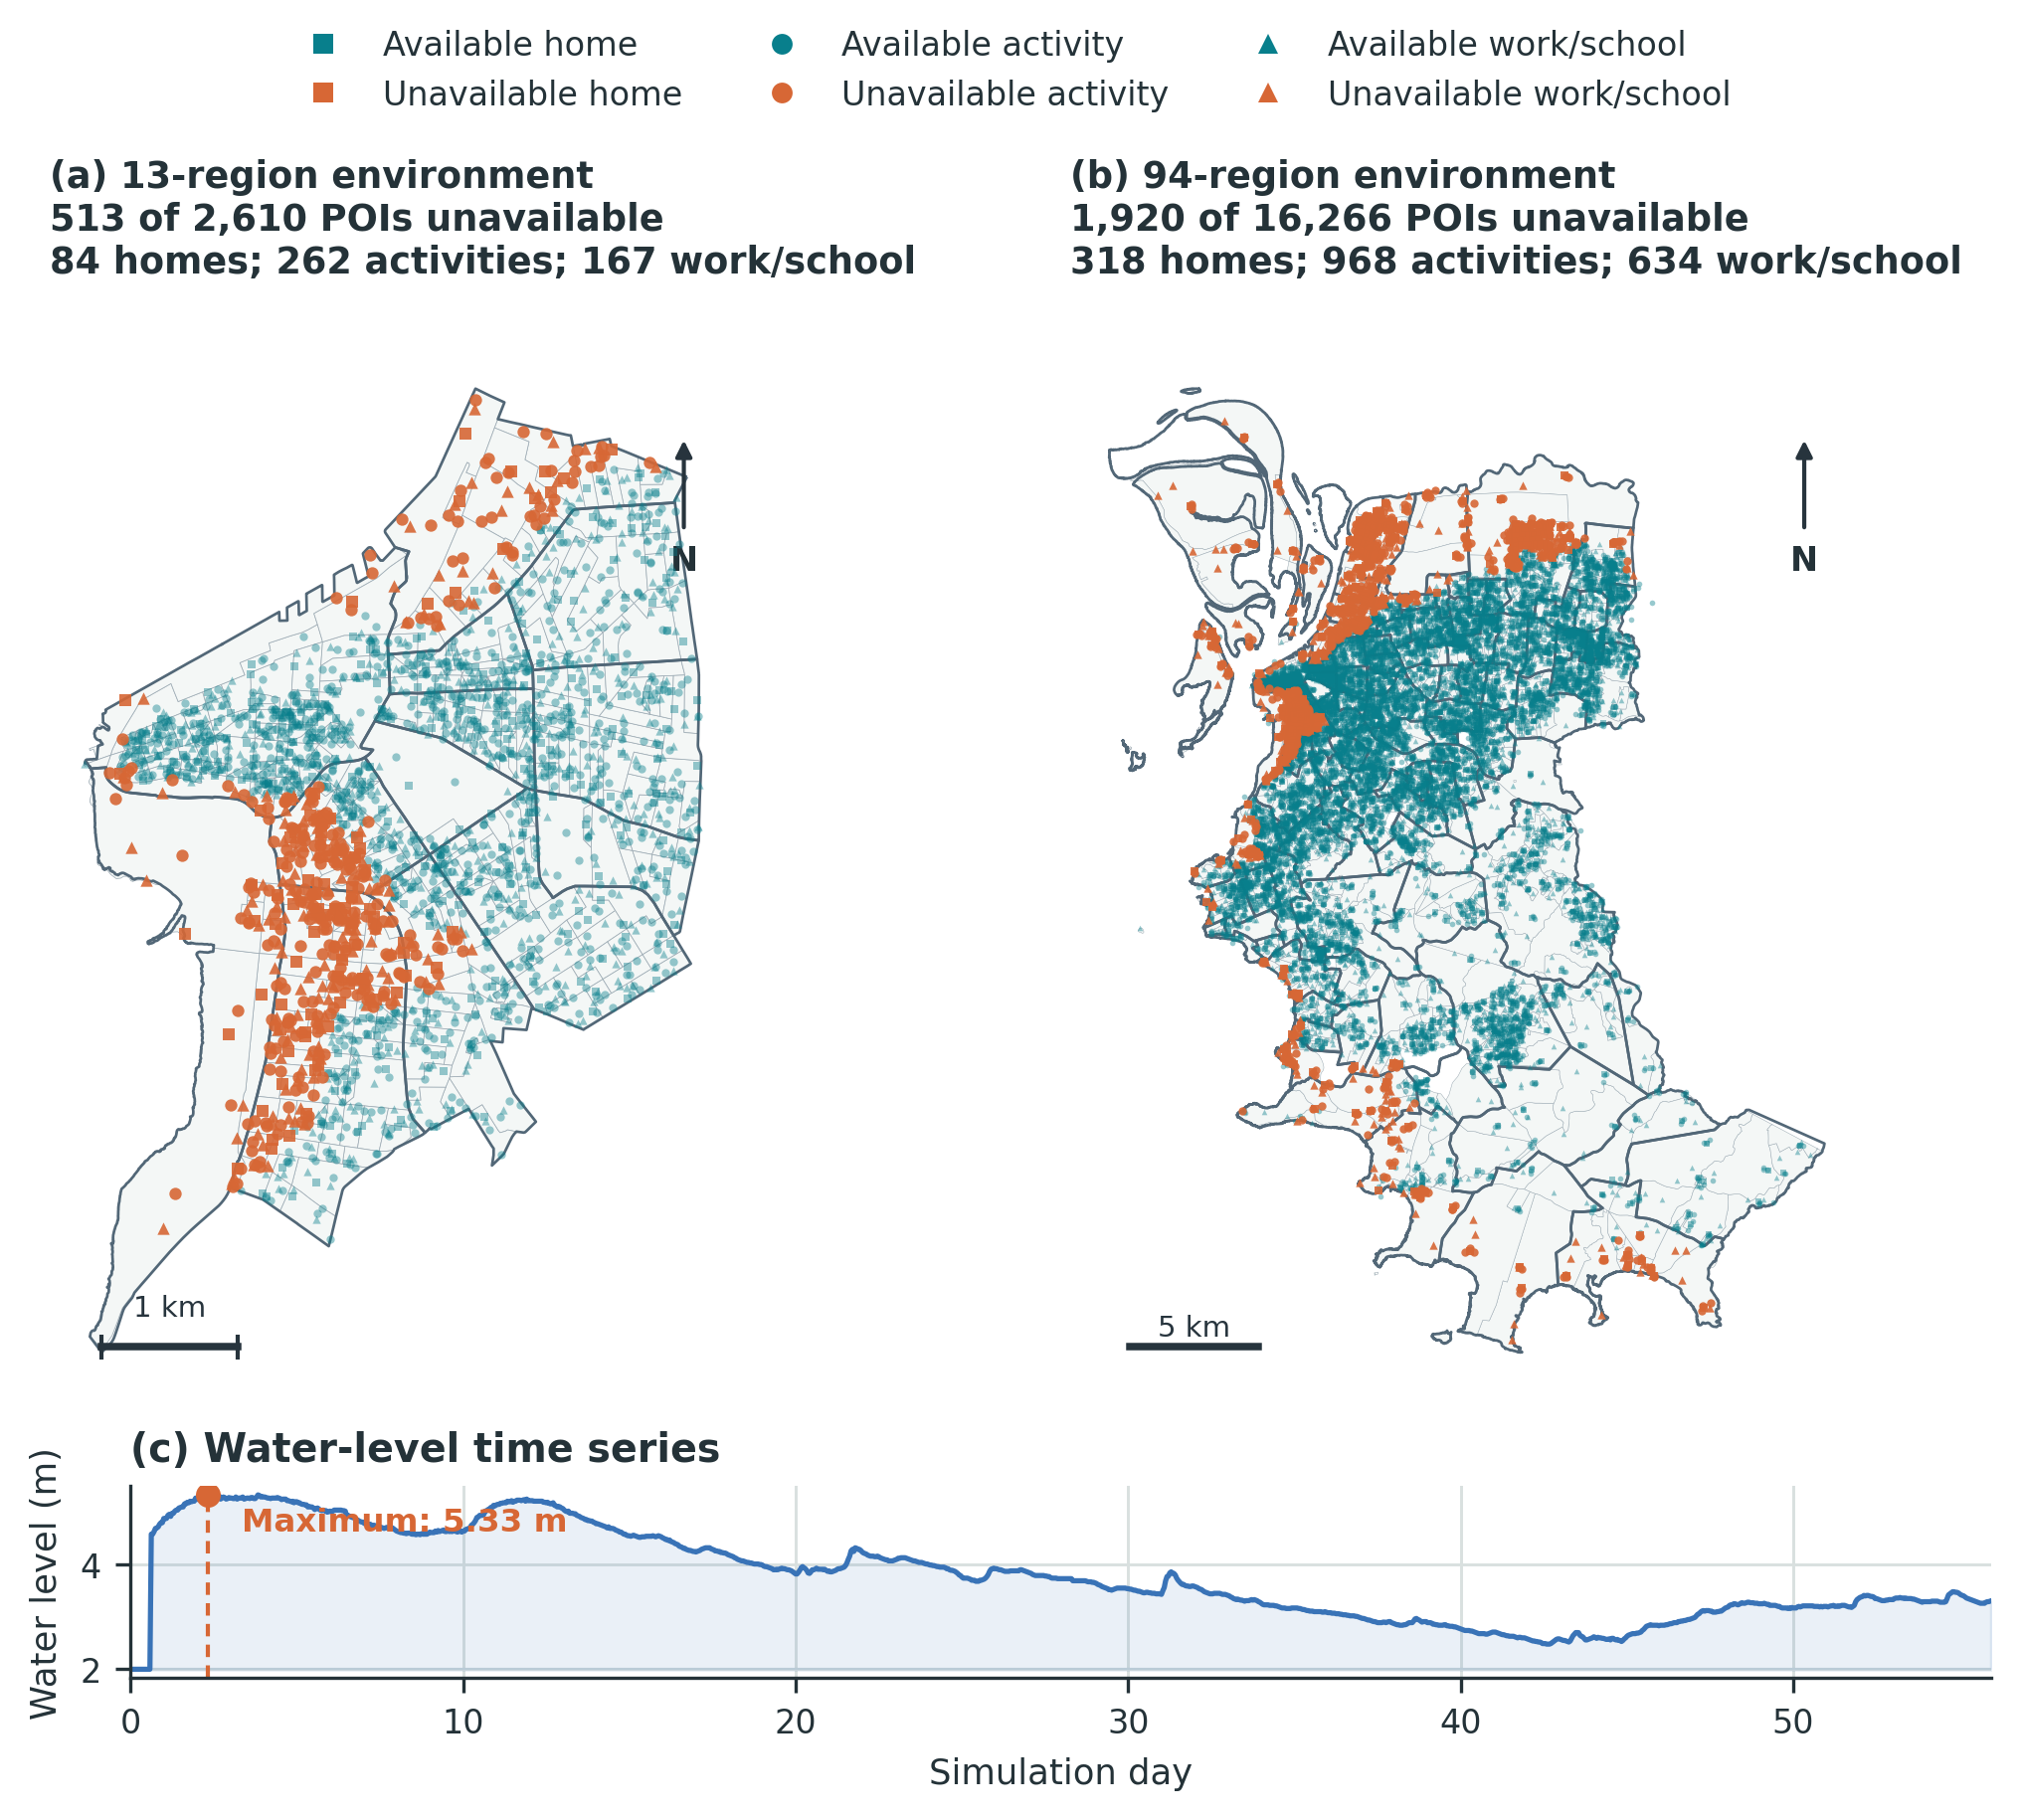
\includegraphics[width=\linewidth]{Figures/environment_disruption_flood_exposure.png}
    \caption{POI availability at the maximum simulated water level in the 13-region and 94-region environments. Marker shape distinguishes homes, activity destinations, and work or school POIs, while color distinguishes available and unavailable states. Panel (c) shows the water-level time series applied during the 56-day simulation.}
    \label{fig:environment_disruption_flood_exposure}
\end{figure}

Table~\ref{tbl:popular_times_disruption} reports Popular Times results with the probabilistic-packet L\'evy Walk configuration enabled. In the 13-region environment, destination exposure suppresses 169,736 of 2,877,888 requested visits, reducing fulfillment from 100\% to 94.10\%. Home exposure preserves fulfillment but increases mean source distance by 12.4716~m relative to the reference. Exposing homes and activity destinations together leaves fulfillment at 94.10\%, showing that unavailable destinations determine the substantive activity-demand loss. In the 94-region environment, destination exposure suppresses 1,212,705 of 23,965,416 requests and reduces fulfillment to 94.94\%. Home exposure alone leaves a mean of only 10 visits unmet but increases mean source distance by 76.5900~m. Combined exposure again produces the same substantive suppression as destination exposure.

\begin{table}[ht]
\centering
\footnotesize
\caption{Popular Times outcomes with the probabilistic-packet L\'evy Walk configuration. The 13-region suppression rows use 30 matched seeds; all 94-region rows and the adaptation rows use five matched seeds.}
\label{tbl:popular_times_disruption}
\begin{tabularx}{\linewidth}{@{}Xrrrr@{}}
\toprule
\textbf{Exposed POIs and policy} &
\shortstack{\textbf{Fulfillment}\\\textbf{(\%)}} &
\textbf{Unmet} &
\shortstack{\textbf{Travelers}\\\textbf{/capita}} &
\shortstack{\textbf{Source distance}\\\textbf{(m)}} \\
\midrule
\multicolumn{5}{@{}l}{\textit{13-region environment}} \\
None
    & 100.00 & 0 & 17.9996 & 82.2457 \\
Activity destinations
    & 94.10 & 169,736 & 16.9380 & 75.5516 \\
Homes
    & 100.00 & 0 & 17.9996 & 94.7172 \\
Homes and destinations
    & 94.10 & 169,736 & 16.9380 & 76.1620 \\
Homes and destinations; reroute
    & 100.00 & 0 & 17.9996 & 81.4164 \\
\addlinespace
\multicolumn{5}{@{}l}{\textit{94-region environment}} \\
None
    & 100.00 & 0 & 18.0000 & 84.0151 \\
Activity destinations
    & 94.94 & 1,212,705 & 17.0891 & 78.8162 \\
Homes
    & 100.00 & 10 & 18.0000 & 160.6051 \\
Homes and destinations
    & 94.94 & 1,212,705 & 17.0891 & 81.6491 \\
Homes and destinations; reroute
    & 100.00 & 5.2 & 18.0000 & 94.8091 \\
\bottomrule
\end{tabularx}
\end{table}

The lower source-distance values under destination suppression are not evidence of improved accessibility. They are calculated only for completed movements: requests whose unavailable destinations would have contributed different trips are omitted. This selection effect occurs in both spatial representations and is why fulfillment and distance must be interpreted together.

Nearest-available, same-type substitution restores all 169,736 suppressed visits in every analyzed 13-region run. The mean displacement between requested and receiving activity destinations is 293.50~m per rerouted traveler. Demand is redistributed among 228 receiving POIs. As detailed in Table~\ref{tbl:popular_times_adaptation_cost}, an active receiver accommodates a mean of 6.60 concurrent rerouted travelers, while the largest rerouted-only concentration is 128 travelers at one restaurant. Relative to the matched five-seed suppression subset, rerouting adds 5.2549~m per requested visit while restoring fulfillment from 94.10\% to 100\%.

In the 94-region environment, substitution fulfills a mean of 1,212,699.8 of the 1,212,705 otherwise suppressed visits, leaving 5.2 unmet requests per run. The requested-to-receiving displacement is 1,174.45~m per rerouted traveler, and 694 POIs receive redirected demand. An active receiver accommodates a mean of 12.77 concurrent rerouted travelers, and the largest rerouted-only concentration is 1,096 travelers at one restaurant. Relative to matched suppression runs, rerouting adds 13.1600~m per requested visit. These results show that the same nearest-available rule produces a larger displacement and greater concentration in the citywide representation; they do not establish that residents would select the same alternatives.

Table~\ref{tbl:popular_times_adaptation_cost} consolidates the adaptation measures for both spatial representations, including the destination-type breakdown and the concurrent load attributable only to rerouted travelers.

\begin{table}[ht]
\centering
\footnotesize
\caption{Activity-destination adaptation costs over five matched runs. The mean concurrent load is calculated over receiver--step combinations with at least one rerouted traveler; the peak excludes travelers who selected the receiving POI directly.}
\label{tbl:popular_times_adaptation_cost}
\begin{tabularx}{\linewidth}{@{}Xrr@{}}
\toprule
\textbf{Measure} & \textbf{13 regions} & \textbf{94 regions} \\
\midrule
Visits requiring substitution & 169,736 & 1,212,705 \\
Rerouted visits fulfilled & 169,736 & 1,212,699.8 \\
Remaining unmet visits & 0 & 5.2 \\
Mean requested-to-receiving displacement (m) & 293.50 & 1,174.45 \\
Receiving marketplaces & 74 & 223 \\
Receiving pharmacies & 75 & 240 \\
Receiving restaurants & 79 & 231 \\
All receiving destinations & 228 & 694 \\
Mean concurrent rerouted load at an active receiver & 6.60 & 12.77 \\
Peak concurrent rerouted load at one receiver & 128 & 1,096 \\
\bottomrule
\end{tabularx}
\end{table}

Enabling the probabilistic-packet L\'evy Walk configuration changes the home populations available when Popular Times requests are sourced, but activity fulfillment is governed primarily by destination availability and the substitution policy. In the 13-region environment it does not change fulfillment, travelers per capita, or occupancy per requested visit within an exposure stratum. The corresponding 94-region results follow the same pattern apart from the negligible mean of 10 unmet visits under home-only exposure. Its principal measured effect in this matrix is therefore on sourcing distance.

\subsubsection{Flood-Aware Work and School Mobility}

The attendance-controlled L\'evy Walk configuration makes work and school demand explicit, allowing attendance to be requested and audited independently of activity visits. Table~\ref{tbl:levy_attendance_disruption} shows that, in the 13-region environment, destination exposure reduces commute fulfillment to 92.47\%, home exposure reduces it to 89.27\%, and exposing all relevant POI types reduces it to 84.89\%. The corresponding values in the 94-region environment are 94.36\%, 93.16\%, and 90.31\%.

\begin{table}[ht]
\centering
\footnotesize
\caption{Mean Popular Times and attendance-controlled L\'evy Walk outcomes over five matched seeds in each environment.}
\label{tbl:levy_attendance_disruption}
\begin{tabularx}{\linewidth}{@{}lrrrX@{}}
\toprule
\textbf{Condition} &
\shortstack{\textbf{Commute}\\\textbf{fulfillment}} &
\shortstack{\textbf{Commute}\\\textbf{unmet}} &
\shortstack{\textbf{Mean distance}\\\textbf{(m)}} &
\textbf{Activity fulfillment} \\
\midrule
\multicolumn{5}{@{}l}{\textit{13-region environment}} \\
No exposure
    & 1.0000 & 2.8 & 1,411.15 & 1.0000 \\
Destinations
    & 0.9247 & 514,114.4 & 1,382.67 & 0.9410 \\
Homes
    & 0.8927 & 733,115.8 & 1,408.29 & 1.0000 \\
All POI types
    & 0.8489 & 1,032,192.2 & 1,364.93 & 0.9410 \\
All POI types; activity reroute
    & 0.8476 & 1,040,775.8 & 1,364.47 & 1.0000 \\
\addlinespace
\multicolumn{5}{@{}l}{\textit{94-region environment}} \\
No exposure
    & 1.0000 & 858.4 & 3,687.91 & 1.0000 \\
Destinations
    & 0.9436 & 3,209,072.4 & 3,505.32 & 0.9494 \\
Homes
    & 0.9316 & 3,892,860.8 & 3,654.26 & 1.0000 \\
All POI types
    & 0.9031 & 5,512,150.6 & 3,423.69 & 0.9494 \\
All POI types; activity reroute
    & 0.9024 & 5,556,421.6 & 3,423.25 & 1.0000 \\
\bottomrule
\end{tabularx}
\end{table}

The shorter mean commute distances under destination and combined exposure again reflect the set of trips that remain feasible, not a travel benefit. In the 13-region environment, destination exposure adds a mean of 514,111.6 units of unmet commute demand and reduces mean distance among completed trips by 28.49~m. Combined exposure adds 1,032,189.4 units of unmet commute demand and reduces the completed-trip mean by 46.22~m. In the 94-region environment, the corresponding increases in unmet demand are 3,208,214.0 and 5,511,292.2, while completed-trip mean distance falls by 182.59~m and 264.22~m, respectively.

Activity rerouting in the combined condition restores Popular Times fulfillment to 100\% in the 13-region environment and leaves only 16.6 mean unmet activity requests in the 94-region environment, which also rounds to 100\%. It does not restore work or school attendance. Commute fulfillment remains 84.76\% and 90.24\%, respectively, and is slightly lower than in the matching activity-suppression conditions. This composed result is consistent with the two plugins drawing from the same represented population while retaining different destination semantics: Popular Times can substitute another POI with the same type $\tau_i$, while L\'evy Walk continues to report the unavailable workplace or school as unmet.



\subsubsection{Shelter Results}

Table~\ref{tbl:shelter_reference_results} presents the principal shelter references. At the end of the reference run, all 12,519 configured places are in use, corresponding to 6.84\% of the 182,936 mapped exposed population. The remaining 170,417 people retain an \texttt{in\_danger} status. Coverage is identical across seeds because the fixed capacity is fully used.

\begin{table}[ht]
\centering
\footnotesize
\caption{Mean shelter outcomes over five seeds. Waiting is accumulated over hourly simulation steps and is therefore reported in person-hours.}
\label{tbl:shelter_reference_results}
\begin{tabularx}{\linewidth}{@{}lrrrrX@{}}
\toprule
\textbf{Policy} &
\shortstack{\textbf{Coverage}\\\textbf{(\%)}} &
\shortstack{\textbf{Unresolved}\\\textbf{demand}} &
\shortstack{\textbf{Peak}\\\textbf{waitlist}} &
\shortstack{\textbf{Waiting}\\\textbf{(million person-h)}} &
\textbf{Mean distance} \\
\midrule
No reallocation
    & 6.843 & 170,417 & 24,195 & 3.998 & 5.511~km \\
Reallocation
    & 6.843 & 170,417 & 24,195 & 3.950 & 5.537~km \\
\bottomrule
\end{tabularx}
\end{table}

Reallocation does not change final coverage or peak waitlist in the reference because the network has no unused capacity once all shelters are full. It does reduce accumulated waiting by 47,813 person-hours, a 1.20\% reduction, while increasing mean travel distance by 0.0267~km.

Table~\ref{tbl:shelter_capacity_response} separates the quantity of shelter space from the rate at which exposed residents attempt to use it. Halving capacity reduces final coverage to 3.42\%. Doubling it raises coverage to 13.69\%, and multiplying it by five raises coverage to approximately 20.07\%. Increasing capacity from five to fifteen times the reference produces essentially no additional protection within 14 days. At this point, capacity is no longer binding: the 1\%-per-day response schedule limits how much of the exposed population reaches shelters during the simulated horizon.

\begin{table}[ht]
\centering
\footnotesize
\caption{Shelter capacity and daily-response sensitivity over five seeds. The reference uses 1$\times$ capacity and a 1\% daily response.}
\label{tbl:shelter_capacity_response}
\begin{tabularx}{\linewidth}{@{}lrrrrX@{}}
\toprule
\textbf{Condition} &
\shortstack{\textbf{Coverage}\\\textbf{(\%)}} &
\textbf{Unresolved} &
\shortstack{\textbf{Peak}\\\textbf{waitlist}} &
\shortstack{\textbf{Waiting}\\\textbf{(million person-h)}} &
\textbf{Binding effect} \\
\midrule
0.5$\times$ capacity & 3.423 & 176,674 & 25,499 & 4.362 & Capacity \\
1$\times$ capacity  & 6.843 & 170,417 & 24,195 & 3.950 & Capacity \\
2$\times$ capacity  & 13.687 & 157,898 & 11,676 & 0.981 & Capacity \\
5$\times$ capacity  & 20.069 & 146,223 & 1,843 & 0.033 & Response horizon \\
15$\times$ capacity & 20.069 & 146,222 & 1,841 & 0.026 & Response horizon \\
\addlinespace
0.5\% response & 6.843 & 170,417 & 11,436 & 1.755 & Slower arrival \\
2\% response   & 6.843 & 170,417 & 49,633 & 8.357 & Faster queuing \\
5\% response   & 6.843 & 170,417 & 124,364 & 21.429 & Faster queuing \\
\bottomrule
\end{tabularx}
\end{table}

Changing the response rate alone does not change final coverage because even the 0.5\% condition eventually fills the reference capacity. It substantially changes congestion: increasing the rate from 0.5\% to 5\% raises the peak waitlist from 11,436 to 124,364 and accumulated waiting from 1.75 million to 21.43 million person-hours. Faster requests are therefore not equivalent to faster protection when admission capacity is fixed.

Exposure scaling produces the corresponding demand-side effect. With 25\% of the reference exposure, coverage reaches 26.85\%, unresolved demand falls to 34,111, and accumulated waiting is 0.643 million person-hours. At 50\% exposure, coverage is 13.42\%, unresolved demand is 80,742, and waiting is 1.721 million person-hours. The 100\% reference returns to 6.84\% coverage and 3.950 million waiting person-hours.

Table~\ref{tbl:shelter_failures} reports the reference and the two retained shelter-failure scenarios with waitlist reallocation enabled.

\begin{table}[ht]
\centering
\footnotesize
\caption{Mean shelter failure outcomes over five seeds. All rows use waitlist reallocation.}
\label{tbl:shelter_failures}
\begin{tabularx}{\linewidth}{@{}>{\raggedright\arraybackslash}Xrrrrl@{}}
\toprule
\textbf{Condition} &
\shortstack{\textbf{Coverage}\\\textbf{(\%)}} &
\textbf{Unresolved} &
\shortstack{\textbf{Mean distance}\\\textbf{(km)}} &
\shortstack{\textbf{P95 distance}\\\textbf{(km)}} &
\textbf{Capacity removed} \\
\midrule
No shelter failure        & 6.843 & 170,417 & 5.537 & 17.699 & None \\
Largest shelter disabled  & 6.573 & 170,912 & 5.522 & 17.714 & 495 places \\
Highest-capacity 10\% of shelters disabled & 4.675 & 174,384 & 5.731 & 17.917 & 3,967 places \\
\bottomrule
\end{tabularx}
\end{table}

Disabling the single largest shelter adds \texttt{shelter\_failure} to its cause set, removes 495 available places, and reduces coverage by 0.271 percentage points. Applying the same cause to the 11 highest-capacity shelters---10\% of the 104-POI shelter network after rounding---removes 3,967 places and reduces coverage by 2.169 percentage points.

Reallocation again changes waiting rather than final coverage in the failure scenarios. It reduces accumulated waiting by 46,546 person-hours after the largest-shelter failure and by 35,265 person-hours after failure of the 11 highest-capacity shelters, while adding approximately 0.027 and 0.030~km to mean travel distance, respectively. Once every remaining enabled shelter is full, no reallocation policy can recover the protection lost with disabled capacity.

\subsection{Remarks}

The results demonstrate why POI state and response policy must remain separate. The Water-Level Data Plugin applies the same \texttt{flood} cause to $C_i(t)$ according to $\bm{\alpha}_i[\mathrm{water\_level}]$, yet the outcomes differ because Popular Times may suppress or substitute an activity destination, attendance-controlled L\'evy Walk records requested work and school demand as unmet, and the Shelter Plugin creates new protection-seeking movement subject to capacity. The framework supports these responses without embedding any one of them in the core POI definition.

Destination substitution is effective only for the demand to which it is applied. The nearest-available, same-type policy restores every suppressed marketplace, restaurant, and pharmacy visit in the 13-region environment and all but a negligible residual in the 94-region environment, but it adds travel and receiving load and does not compensate for unavailable workplaces or schools. Similarly, shelter reallocation uses distributed spare capacity and reduces waiting exposure, but it cannot replace failed or insufficient capacity. Coverage, unmet demand, waiting, distance, and receiving load therefore capture distinct effects and should be reported together.

The shelter results further show that capacity and response speed are joint constraints. Under reference capacity, faster evacuation requests mainly create longer queues. Under sufficiently expanded capacity, the 14-day response schedule limits final protection. Failure consequences depend on how much capacity is removed and where shelters exist, rather than solely on the number of affected regions.

These results remain conditional on the implemented assumptions. Water thresholds in $\bm{\alpha}_i$, plugin parameters in $\bm{\theta}_{\Pi}$, hourly activity profiles, same-type nearest substitution, commute attendance rates, exposure multipliers, shelter capacities, response rates, and failure selections are experiment inputs. Mobility uses geographic rather than transport-network distance. Except for the 30-seed 13-region suppression matrix, the mobility comparisons reported here use five seeds and should be interpreted as screening estimates. The shelter workflow models static initial exposure, simple capacity admission, and no demographic priority, recovery, or return-home decision. Its five-seed catalog is likewise a screening analysis of stochastic evacuation outcomes, not an exhaustive uncertainty analysis or a forecast of observed evacuation behavior. Because $D_i$ is empty for the POIs in this section, the experiments evaluate direct disable causes and plugin responses; dependency propagation is evaluated separately by the subsequent dialysis experiments.
